\section{Results}

Let's take a circular domain (radius $R=1$) for example to apply the method. To validate it, we take the position of the source at given coordinates $(x_0, y_0)$ and we excute the program to see if it is able to find the position of the source by iterating the algorithm with calculated coordinates $(x_n, y_n)$.\\
We first noticed that depending on the position of the source the calculation took more or less time and that we could impact the time of calculation by adjusting the parameter alpha of the algorithm. As said before we have a function that modifies alpha depending on the magnitude of the gradient norm. \\

\subsection{First test case}

For the first test case, we take $(0.5, 0.5)$ as the coordinates of the source. \\
\begin{figure}[H]
	\centering
	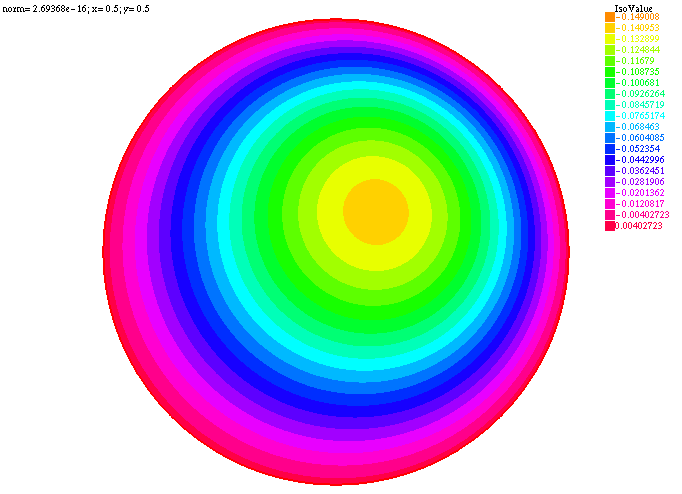
\includegraphics[scale=0.7]{0505.png}
	\caption{Converged solution of source position}
	\label{0505}
\end{figure}
We can see on figure \ref{0505} that the position has been found by the algorithm (top left corner) and the colors represent the values of the function $\phi$ where the maximum is on the source as expected.

Let's see how many iterations it takes for the  loop to converge with a convergence criteria of $10^{-16}$.\\
\begin{center}
$\begin{array}{|c|c|}
	\hline
	\text{Number of points} & \text{Iterations} \\
	\hline
	40 & 45\\
	80 & 46\\
	160 & 45 \\
	320 & 46\\
	\hline
\end{array}$
\end{center}

As we can see, the number of iterations needed to converge do not depends on the size of the mesh.

\subsection{Second test case}

For the second test case, we take $(0.95,0)$ as the coordinates of the source.\\
\begin{figure}[H]
	\centering
	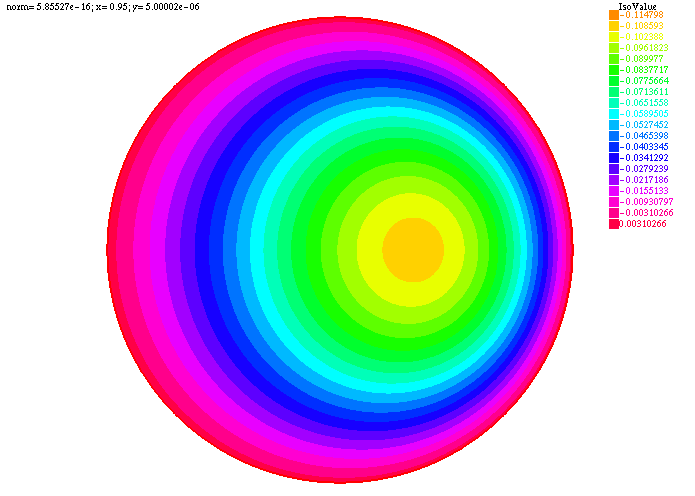
\includegraphics[scale=0.7]{0950.png}
	\caption{Converged solution of source position}
	\label{0950}
\end{figure}
On the top left corner we can see that the position of the source has been found. However the maximum of the function $\phi$ is not at this position. This is because we have a boundary condition that impose $\left.\Phi\right|_{\partial\Omega}=0$.

 